\documentclass{cours}
\usepackage{pgfplots}
\usepackage{multicol}
\usepackage{cases}
\usepackage{calc}
%\usepackage{esvect}
\usepackage{tikz-3dplot} 
\usetikzlibrary{patterns}
\usetikzlibrary{decorations.text}

\begin{document}
\setcounter{chapter}{12}
\chapter{Mouvement de particules chargées}
Dans ce chapitre, on étudiera le mouvement de particules chargées ponctuelles soumises à des champs électriques ou magnétiques indépendants du temps (électrostatique, magnétostatique) et uniformes (identiques en tout point de l'espace)

\section{Force de Lorentz}%
\label{sec:force_de_lorents}
La résultante des forces électrique et magnétique s'appelle la force de Lorentz, elle se décompose en une composante électrique et une composante magnétique.

\subsection{Champs électrique et magnétique}%
\label{sub:force_electrique}
Les effets des interactions électriques et magnétiques entre particules sont modélisés par l'existence des champs électriques et magnétiques notés respectivement $\vv{E}$ et $\vv{B}$. 

Dans le cas général ces champs dépendent du temps et du points de l'espace où l'on se trouve mais dans ce chapitre nous ne considérerons que des champs uniformes et stationnaires. Chacun sera donc entièrement défini par un vecteur unique.    

\subsection{Force de Lorentz}%
\label{sub:force_de_lorentz}
\begin{loi}{Force de Lorentz}
Une particule $M$ ponctuelle de charge $q$ et de vitesse $\vv{v}$ dans le référentiel d'étude, plongée dans des champs électrique $\vv{E}$ et magnétique $\vv{B}$, subit une force appelée \emph{force de Lorentz} 
\begin{equation}
  \vv*{F}{L} = q\vv{E} + q\vv{v}\wedge\vv{B} \, .
\end{equation}
\end{loi}
% 
Elle comporte deux composantes :
\begin{itemize}
  \item Une composante électrique $\vv*{F}{e} = q \vv{E}$ ;
  \item une composante magnétique $\vv*{F}{m} = q\vv{v}\wedge \vv{B}$. 
\end{itemize}

On peut comparer l'intensité de l'attraction électrostatique $F_e$ entre deux électrons à celle de leur interaction gravitationnelle $F_g$. On a pour deux électrons séparés d'une distance $r$ 
\begin{equation}
  F_e = \frac{e^2}{4\pi\varepsilon_0r^2}
\end{equation}
et
\begin{equation}
  F_g = G\frac{m_e^2}{r^2}\, .
\end{equation}
Le rapport de ces deux forces est :
\begin{equation}
  \frac{F_e}{F_g} = \frac{e^2}{4\pi\varepsilon_0m_e^2G} \approx \luaexec{SIe(_e^2/(4*math.pi*_e_0*_m_e^2*_G), 0, "")}
\end{equation}

Comparons également la force magnétique $F_m$  subie par un électron se déplaçant à une vitesse de \SI{1}{\meter\per\second} dans le champ magnétique terrestre à son poids $P$. On a 
\begin{equation}
  F_m = evB \quad \text{et} \quad P = m_eg\, .
\end{equation}
Dans ces conditions
\begin{equation}
 \frac{F_m}{P} = \frac{evB}{m_eg} \approx \luaexec{SIe(_e*50e-6*1/_m_e/_g, 0, "")}
\end{equation}
Dans ces deux cas, on remarque que les forces électrostatique et magnétostatique sont très largement supérieures aux forces gravitationnelles. Dans la vaste majorité des situations, on pourra négliger la force de gravitation par rapport à la force de Lorentz.

\subsection{Puissance de la force de Lorentz}%
\label{sub:puissance_de_la_force_de_lorentz}
La puissance fournie par la force de Lorentz est 
\begin{equation}
P = \vv*{F}{L}\cdot \vv{v} = q \vv{E}\cdot \vv{v} + \underbrace{q \vv{v}\wedge \vv{B}\cdot \vv{v}}_{=0} = q \vv{E}\cdot \vv{v}
\end{equation}
Le terme magnétique est toujours nul car $\vv{v}\wedge \vv{B}$ est toujours perpendiculaire à $\vv{v}$ et le produit scalaire est nul.

Un champ magnétique ne peut donc pas fournir d'énergie à une particule chargée, il peut uniquement courber sa trajectoire (la force est perpendiculaire à la trajectoire). 

Un champ électrique est, au contraire, capable de modifier l'énergie cinétique d'une particule.

Déterminons le travail fourni par la force de Lorentz à une particule chargée entre deux points $A$ et $B$. Un point matériel $M$ de charge $q$ soumis uniquement à la force électrostatique $\vv{F} = q\vv{E}$ entre $A$ et $B$. Le travail de la force de Lorentz entre les points $A$ et $B$ est 
\begin{equation}
W_{AB} = \int_A^B\vv{F}\cdot\D \vv{u} = \int_A^B q\vv{E}\cdot\D \vv{u} = q\vv{E}\cdot\int_A^B\D\vv{u} = q\vv{E}\cdot\vv{AB}
\end{equation}

Donc $W_{AB}$ est indépendant du chemin suivi entre $A$ et $B$. On dit que le poids est une \textbf{force conservative}.

On peut écrire $W_{AB}$ de la manière suivante :
\begin{center}
  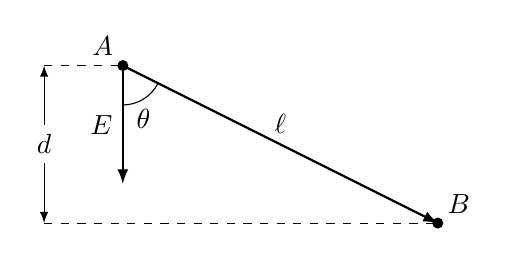
\begin{tikzpicture}
    \coordinate (A) at (0,0);
    \coordinate (B) at (4,-2);
    \fill (A) circle(2pt) node[above left] {$A$ };
    \fill (B) circle(2pt) node[above right] {$B$ };
    \draw[-latex, thick] (A) -- ++(0, -1.5) node[midway, left]{$\vv{E}$} ;
    \draw[-latex, thick] (A) --  (B) node[above, midway]{$\ell$} ;
    \draw (0, -0.5) arc(-90:-{atan(1/2)}:0.5) node[below, midway]{$\theta$};
    \draw[dashed] (-1, 0) -- (0,0); 
    \draw[dashed] (-1, -2) -- (4,-2); 
    \draw[latex-latex] (-1, 0) -- (-1, -2) node[midway, fill=white]{$d$ };
  \end{tikzpicture}
\end{center}

\begin{equation}
W_{AB} = qE\ell\cos(\theta) = qEd = qU_{AB} = qV_A-qV_B 
\end{equation}

La quantité $qV$ est l'\textbf{énergie potentielle électrostatique} du point $M$. $V_A$ et $V_B$ désignent le \textbf{potentiel électrostatique} aux points $A$ et $B$.  
\section{Champ électrostatique uniforme}%
\label{sec:mouvement_dans_un_champ_electrique_uniforme}

Considérons une particule $M$ de charge $q$ plongée dans un champ électrique uniforme et stationnaire $\vv{E} = E \vex$. On ne considère que la force de Lorentz en négligeant les autres forces.

Le principe fondamental de la dynamique appliquée à la particule $M$ dans un référentiel galiléen donne 
\begin{equation}
m\vv{a} = q\vv{E} = qE \vex \Leftrightarrow 
\begin{cases}
  \ddot{x} = \frac{qE}{m}\\
  \ddot{y} = 0 \\
  \ddot{z} = 0
\end{cases}
\Leftrightarrow
\begin{cases}
  x(t) = \frac{qE}{2m}t^2 + v_{0x}t + x_0\\
  y(t) = v_{0y}t + y_0\\
  z(t) = v_{0z}t + z_0
\end{cases}
\end{equation}
Il s'agit donc d'un mouvement uniformément accéléré suivant l'axe $x$, que l'on a déjà étudié dans le chapitre précédent. C'est l'équivalent d'une chute libre dans le champs de pesanteur terrestre. 

On peut déterminer la vitesse d'une particule de charge $q$ accélérée par une différence de potentielle $U$ en utilisant le théorème de l'énergie cinétique :
\begin{equation}
  \Delta E_c =\frac{1}{2}m(v_B^2-v_A^2)= W_{AB}(\vv{F}) = qU_{AB}
\end{equation}
Si la vitesse initiale de la particule est nulle ($v_A=0$) on obtient 
\begin{eqencadre}
  v_B = \sqrt{\frac{2qU_{AB}}{m}}
\end{eqencadre}
Pour un électron accéléré sous une différence de potentiel de \SI{100}{\kilo\volt}, on obtient une vitesse finale de 
\begin{equation}
  v = \sqrt{\frac{2eU}{m}} \approx \luaexec{SIe(math.sqrt(2*_e*100e3/_m_e), 2, "\\meter\\per\\second")}
\end{equation}
C'est une vitesse qui est proche de la vitesse de la lumière dans le vide, on dit que la particule est \emph{relativiste} et ce mode de calcul de la vitesse n'est plus adapté, il faut utiliser la relativité restreinte.

L'expression de l'énergie cinétique en relativité restreinte est 
\begin{equation}
  E_c = (\gamma-1) mc^2 \quad \text{avec}\quad \gamma = \frac{1}{\sqrt{1-\left(\frac{v}{c}\right)^2}}
\end{equation}
En utilisant cette expression, la vitesse atteinte par la particule devient 
\begin{equation}
  v = c \sqrt{1-\frac{1}{\left(1+\frac{\Delta E_c}{mc^2}\right)^2}} \approx  \luaexec{SIe(_c*math.sqrt(1-1/(1+_e*100e3/(_m_e*_c^2))^2), 2, "\\meter\\per\\second")}
\end{equation}

L'accélération d'électrons par un champ électrique est utilisé pour produire des faisceaux d'électrons dans les microscopes électroniques, dans certains accélérateurs de particules, dans les expériences de diffraction d'électrons\ldots

\section{Champ magnétostatique uniforme}%
\label{sec:mouvement_dans_un_champ_magetostatique_uniforme}
On s'intéresse maintenant au mouvement d'une particule $M$ de charge $q$ dans un champ magnétique uniforme $\vv{B} = B\vez$. On suppose que la vitesse initiale de la particule est perpendiculaire au champ magnétique $\vv*{v}{0} = v_0 \vex$. \footnote{Le résultat reste malgré tout très général, si la vitesse initial n'est pas suivant l'axe $x$, on peut changer de repère et placer un axe $x'$ colinéaire à la vitesse initiale} On considérera également qu'à $t=0$ la particule se trouve à l'origine du repère. 

\begin{center}
  \begin{tikzpicture}
    \draw[-Stealth] (-4,0) -- (4,0) node[right] {$x$};
    \draw[-Stealth] (0,-2) -- (0,2) node[right] {$y$};
    \fill (0,0) circle (2pt) node[above left]{$M$}; 
    \draw[-Stealth, thick] (0,0) -- ++(2,0) node[below, midway] {$\vv*{v}{0}$};
    \fill (3,1) circle (1pt);
    \draw (3,1) circle (5pt);
    \draw (3,1) ++ (45:5pt) node[above right] {$\vv{B}$}; 
  \end{tikzpicture}
\end{center}



La force subie par la particule chargée est
\begin{equation}
  \vv{F} = q \vv{v}\wedge \vv{B} = q
  \begin{pmatrix}
    \dot{x}\\\dot{y}\\\dot{z}
  \end{pmatrix}\wedge
  \begin{pmatrix}
    0\\0\\B
  \end{pmatrix}
  =
  \begin{pmatrix}
   qB \dot{y}\\
   -qB \dot{x}\\
   0
  \end{pmatrix}
\end{equation}
Le principe fondamental de la dynamique donne 
\begin{equation}
  m\vv{a} = \vv{F} \Leftrightarrow 
  \begin{pmatrix}
    m \ddot{x}\\
    m \ddot{y}\\
    m \ddot{z}
  \end{pmatrix}=
  \begin{pmatrix}
    qB \dot{y}\\
    -qB \dot{x}\\
    0
  \end{pmatrix}
\end{equation}
Suivant l'axe $z$, la particule a une accélération nulle, et comme sa vitesse initiale dans cette direction est nulle, la coordonnée $z$ de la particule est constante. On s'intéressera donc uniquement au mouvement dans le plan $(x, y)$. On a les deux équations différentielles
\begin{equation}
  \begin{cases}
    \ddot{x} = \frac{qB}{m}\dot{y}\\
    \ddot{y} = -\frac{qB}{m}\dot{x}
  \end{cases}
\end{equation}
Donc finalement,
  \begin{subnumcases}{}
    \ddot{x} = \omega_c \dot{y} \label{eq:cyclox}\\
    \ddot{y} = -\omega_c  \dot{x}\label{eq:cycloy}
  \end{subnumcases}
où $\omega_c = \frac{qB}{m}$ est la \emph{pulsation cyclotron}. On commence par intégrer l'équation~\eqref{eq:cycloy} entre $0$ et $t$ 
\begin{equation}
  \int_0^t \ddot{y}(t')\, \D t' = -\omega_c \int_0^t \dot{x}(t') \, \D t' \Leftrightarrow \dot{y}(t)  - \underbrace{\dot{y}(0)}_{=0}  = -\omega_c \big( x(t) - \underbrace{x(0)}_{=0} \big) \Leftrightarrow \dot{y}(t) = -\omega_c x(t) 
\end{equation}
%
En introduisant cette expression dans l'équation~\eqref{eq:cyclox} on obtient:
\begin{eqencadre}
  \ddot{x} + \omega_c^2x = 0
\end{eqencadre}
C'est l'équation d'un oscillateur harmonique de pulsation $\omega_c$, dont on connait la solution :
\begin{equation}
  x(t) = A\cos(\omega_c t) + B\sin(\omega_c t)
\end{equation}
en utilisant les conditions initiales $x(0)=0$ et $\dot{x}(0)=v_0$, on trouve $A=0$ et $B=\frac{v_0}{\omega_c}$. Et finalement
\begin{equation}
  x(t) = \frac{v_0}{\omega_c}\sin(\omega_ct)
\end{equation} 
L'équation~\eqref{eq:cycloy} devient alors
\begin{equation}
  \ddot{y} = -v_0\omega_c\cos(\omega_c t) 
\end{equation}
que l'on peut intégrer une première fois en tenant compte du fait que $\dot{y}(0)=0$ pour trouver
\begin{equation}
  \dot{y} = -v_0\sin(\omega_c t)
\end{equation}
puis une seconde fois, avec $y(0) = 0$ pour obtenir
\begin{equation}
  y(t) = \frac{v_0}{\omega_c}\left[\cos(\omega_c t)-1\right]
\end{equation}
L'équation de la trajectoire est donc 
\begin{eqencadre}
  \begin{cases}
    x(t) = \frac{v_0}{\omega_c}\sin(\omega_c t)\\
    y(t) = \frac{v_0}{\omega_c}\left[\cos(\omega_c t)-1\right]
  \end{cases}
\end{eqencadre}
C'est l'équation paramétrique d'un cercle de centre $(0, -\frac{v_0}{\omega_c})$ et de rayon $\frac{v_0}{\omega_c}$. 

\begin{center}
  \begin{tikzpicture}
    \draw[-Stealth] (-4,0) -- (4,0) node[right] {$x$};
    \draw[-Stealth] (0,-3.2) -- (0,1) node[right] {$y$};
    \fill (0,0) circle (2pt) node[above left]{$M$}; 
    \draw[-Stealth, thick] (0,0) -- ++(2,0) node[above, midway] {$\vv*{v}{0}$};
    \fill (3,1) circle (1pt);
    \draw (3,1) circle (5pt);
    \draw (3,1) ++ (45:5pt) node[above right] {$\vv{B}$}; 
    \draw[thick,
          postaction=decorate, 
          decoration={
          markings, 
          mark=at position 1 with{\arrowreversed{stealth}}
          }
          ] (0, -1.5) circle (1.5cm);
    \draw[<->] (0, -1.5) -- ++(-45:1.5) node[midway, fill=white]{$ \frac{v_0}{\omega_c}$ };
  \end{tikzpicture}
\end{center}

Il est à noter que la détermination complète de la trajectoire, telle que nous venons de la faire, n'est pas au programme de MPSI. Il faut cependant être capable de déterminer le rayon de la trajectoire en admettant que celle-ci est circulaire.

Pour cela on commence par rappeler que la force magnétique ne peut pas modifier l'énergie cinétique de la particule et donc la norme de la vitesse reste constante. La trajectoire est donc circulaire uniforme. Dans ce conditions, on sait que l'accélération est uniquement normale et vaut 
\begin{equation}
  a_N = \frac{v_0^2}{R} 
\end{equation}
où $v_0$ est la norme de la vitesse initiale. Le principe fondamentale de la dynamique indique que cette accélération est égale à la norme de la force appliquée à la particule divisée par sa masse :
\begin{equation}
  \frac{v_0^2}{R} = \frac{qv_0B}{m}
\end{equation}
On en déduit directement le rayon de la trajectoire

\begin{eqencadre}
  R = \frac{v_0m}{qB} = \frac{v_0}{\omega_c}
\end{eqencadre}
Ce qui correspond bien au résultat obtenu par la méthode précédente. On pourrait également \emph{deviner} l'expression de $R$ par analyse dimensionnelle. Pour ça il peut être utile de se rappeler de l'expression de la pulsation cyclotron $\omega_c=\frac{qB}{m}$. 

La déviation de la trajectoire de particules chargées par un champ magnétique est utilisé dans les accélérateurs de particules circulaires (CERN, cyclotron, synchrotron, \ldots)

\end{document}
